 \documentclass[12pt]{article}

\usepackage[margin=1.9cm, letterpaper]{geometry}
\usepackage[utf8]{inputenc}
\usepackage{listings}
\usepackage{xcolor}
\usepackage{graphicx}
\usepackage{indentfirst}
\usepackage{tikz}
\usepackage{float}
\usepackage{fancyvrb}
\usepackage{subcaption}
\usepackage{pdfpages}

\usepackage{subfiles}

\usepackage{parskip}
\setlength{\parskip}{1em}
\setlength{\parindent}{2em}

\renewcommand{\thesection}{}
\renewcommand{\thesubsection}{}

\lstdefinestyle{mystyle}{
    basicstyle=\ttfamily\footnotesize,
    tabsize=4
}

\usetikzlibrary{shapes.geometric, arrows}

\tikzstyle{every node}=[font=\scriptsize]

\tikzstyle{terminal} = [rectangle, rounded corners, minimum width=2cm, minimum height=1cm,text centered, draw=black, text width=4.5em]
\tikzstyle{process} = [rectangle, text badly centered, minimum width=3cm, draw=black, text width=5em, node distance=3.5cm]
\tikzstyle{decision} = [diamond,aspect=2, minimum width=1cm,text badly centered, draw=black, text width=6em, node distance=2cm]
\tikzstyle{io} = [trapezium, trapezium left angle=70, trapezium right angle=110, text centered, draw=black, text width=5em]
\tikzstyle{arrow} = [thick,->,>=stealth]

\begin{document}
\begin{titlepage}
    \begin{center}
    \vspace*{1cm}
    
    \textbf{Lab 1}

    \vspace{0.5cm}

    Introduction to Assembly Language            
    \vspace{1.5cm}

    \textbf{Hans Jarales (1537516) and Michael Kwok (1548454)}

    \vfill
            
    ECE 212 Lab - Introduction to Microprocessors\\
    Department of Electrical and Computer Engineering\\
    University of Alberta\\
    5 February 2020

   \end{center}
\end{titlepage}

\tableofcontents
\pagebreak

\section{Introduction}
    In this lab, we explore basic programming in assembly language, specifically ColdFire assembly. The basic instruction set (\Verb#move, movea, add, sub, etc#) are used in tandem with comparison and branching to achieve the same functionality analogous to \Verb#if-else# statements used in other high-level programming languages. The purpose and operation of the programs were first conceptualized through the use of flowcharts (Figure 1). Further explored is the functionality of the NetBurner Eclipse IDE in connection with the ColdFire board. Running the programs, and debugging them were performed utilizing this development environment.

\section{Design}
\subsection{Part A}
    In Part A, the program converts an ASCII character to the hexadecimal equivalent, i.e. \Verb#'A' = 0xA#, \Verb#'9' = 0x9#. If the ASCII character is not between 0-9, A-Z or a-z, the program will place an error code at the corresponding memory location. When the program reads the ASCII \Verb#'CR', 0x0D#. The program starts looking for data at the address \Verb#0x43000000#, storing the converted data in \Verb#0x43100000#. Address Registers \Verb#A1# and \Verb#A2# were used to store the addresses in the code.
    
    A loop and switch-case structure is used for the program. The address registers are initialized first, and the comparison is ran. Afterwards, there is a post loop section that gets run that increments the address registers before doing the checks again.
    
    In the code, the first case checked is if the content of the memory address is \Verb/0x0D/. If it is, the program stops. If it isn't, the data is tested to see if it's $\geq0$. If it's less than 0, it's an error. Next, the program checks to see if the data is $\geq$\Verb/0x41/. If it is, the 5th bit gets ORed to force the data to be in the lower case a-z, making the comparison simpler.

    
    \begin{lstlisting}[language={[Motorola68k]Assembler}, style={mystyle}]
    Conversion Example
    
    D2 = 'A' = 0x41 = 0b01000001    /* D2 initially has ASCII 'A' */

    OR.L #0x20, D2                  /* 5th bit is kept on */
    /* -> D2 = 0b01100001 = 0x61 = 'a'  Result is ASCII 'a' */
    AND.L #15, D2
    /* D2 = 0b00000001 = 0x1 */
    ADD.L #0x9, D2
    /* D2 = 0xA */
    \end{lstlisting}

\subsection{Part B}
    This program converts an ASCII letter from uppercase to lowercase, and vice versa. An ASCII character that is not a letter returns error code 0xFFFFFFFF. When the program reads ASCII 'ENTER' (0xD), the program stops.The ASCII uppercase characters range from 0x41 (A), to 0x5A (Z). The lowercase characters range from 0x61 (a), to 0x7A (z). Outside of these intervals, the ASCII character must then be a non-letter. Data to be checked comes from memory location starting at 0x43000000. The results of the program are sent to memory locations starting at 0x43200000. In this program, a2, and a3 are used as pointers to these memory locations, respectively.

    A loop is initiated to perform the following operations: the program reads the memory location(s) using the address register pointer (a2) starting at 0x43000000, and first must confirm if the data obtained is \Verb#ENTER 0xD# before performing other checks and conversions. The program then checks if the data is within the intervals of uppercase/lowercase letters. If not, the \Verb#Error code 0xFFFFFFFF# is returned. If a letter is confirmed, a conversion is performed by toggling the fifth bit of the ASCII letter (EOR.L \#0x20, (a2)). Finally, after storing the results, the address pointers are incremented and the loop reruns. Since the data is given in 32-bit format, the address pointers are incremented by 4.
    
    \begin{lstlisting}[language={[Motorola68k]Assembler}, style={mystyle}]
    Conversion Example
    
    D2 = 'A' = 0x41 = 0b01000001    /* D2 initially has ASCII 'A' */

    EOR.L #0x20, D2                 /* 5th bit is toggled */
    /* -> D2 = 0b01100001 = 0x61 = 'a'  Result is ASCII 'a' */
    \end{lstlisting}
    
        \begin{figure}[H]
            \begin{subfigure}{0.5\textwidth}
             \resizebox{\textwidth}{!}{
        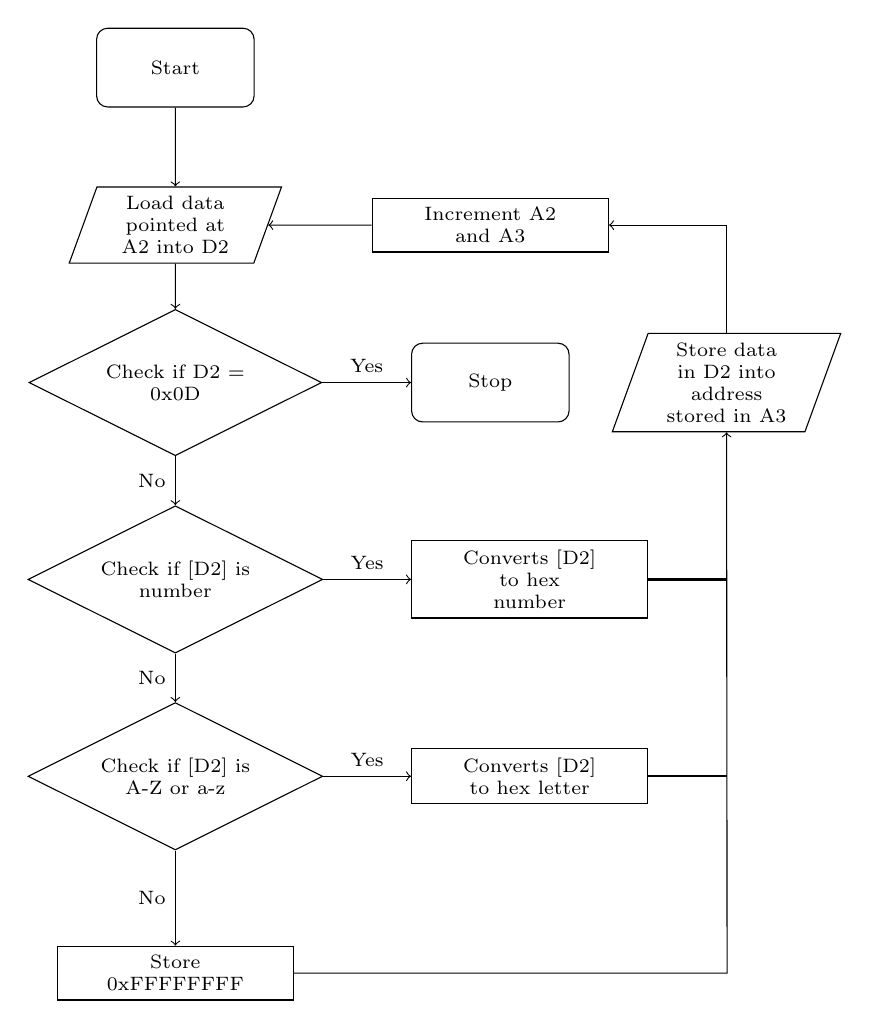
\begin{tikzpicture}[node distance = 2cm]

        \node (start) [terminal] {Start};

        \node (memoryread) [io, below of=start] {Load data pointed at A2 into D2};
        \node (entercheck) [decision, below of=memoryread] {Check if D2 = 0x0D};

        \node (numbercheck) [decision, below of=entercheck, yshift=-0.5cm] {Check if [D2] is number};
        \node (lettercheck) [decision, below of=numbercheck, yshift=-0.5cm] {Check if [D2] is A-Z or a-z};

        \node (processnumber) [process, right of=numbercheck, xshift=1cm] {Converts [D2] to hex number};
        \node (processletter) [process, right of=lettercheck, xshift=1cm] {Converts [D2] to hex letter};

        \node (stop) [terminal, right of=entercheck, xshift=2cm] {Stop};

        \node (savedata) [io, right of=stop, xshift=1cm] {Store data in D2 into address stored in A3};
        \node (increment) [process, above of=stop, yshift=-1.5cm] {Increment A2 and A3};
        \node (error) [process, below of=lettercheck, yshift=1cm] {Store 0xFFFFFFFF};

        \coordinate [right of=processnumber] (hub) {};

        \draw[->] (start) -- (memoryread);
        \draw[->] (memoryread) -- (entercheck);

        \draw[->] (entercheck) -- node[anchor=south] {Yes} (stop);
        \draw[->] (entercheck) -- node[anchor=east] {No} (numbercheck);
        \draw[->] (numbercheck) -- node[anchor=east] {No} (lettercheck);
        \draw[->] (lettercheck) -- node[anchor=east] {No} (error);

        \draw[->] (numbercheck) -- node[anchor=south] {Yes} (processnumber);
        \draw[->] (lettercheck) -- node[anchor=south] {Yes} (processletter);

        \draw[thick] (processnumber.east) -- ++ (1cm,0);
        \draw[thick] (processletter.east) -- ++ (1cm,0);
        \draw[->] (error.east) -- ++ (5.5cm,0) -- (savedata.south);
        \draw[->] (savedata) |- (increment);
        \draw[->] (increment) -- (memoryread);

        \end{tikzpicture}}
        \caption{Flowchart of Part A}
        \end{subfigure}
    \begin{subfigure}{0.4\textwidth}
    \resizebox{\textwidth}{!}{
    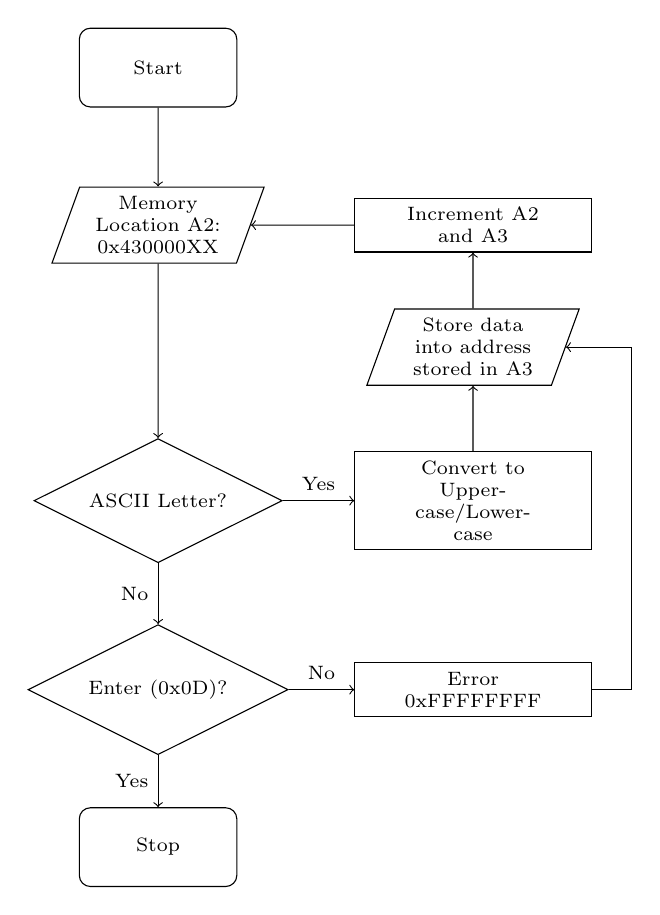
\begin{tikzpicture}[node distance = 2cm]

        \node (start) [terminal] {Start};
        \node (memoryread) [io, below of=start] {Memory Location A2: 0x430000XX};
        \node (lettercheck) [decision, below of=memoryread, yshift=-1.5cm] {ASCII Letter?};
        \node (entercheck) [decision, below of=lettercheck, yshift=-0.4cm] {Enter (0x0D)?};
        \node (processletter) [process, right of=lettercheck, xshift=0.5cm] {Convert to Uppercase/Lowercase};
        \node (stop) [terminal, below of=entercheck] {Stop};
        \node (increment) [process, right of=memoryread, xshift=0.5cm] {Increment A2 and A3};
        \node (savedata) [io, below of=increment, yshift=0.45cm] {Store data into address stored in A3};
        \node (error) [process, right of=entercheck, xshift=0.5cm] {Error 0xFFFFFFFF};

        \draw[->] (start) -- (memoryread);
        \draw[->] (memoryread) -- (lettercheck);
        \draw[->] (lettercheck) -- node[anchor=east] {No} (entercheck);
        \draw[->] (entercheck) -- node[anchor=east] {Yes} (stop);
        
        \draw[->] (lettercheck) -- node[anchor=south] {Yes} (processletter);
        \draw[->] (entercheck) -- node[anchor=south] {No} (error);
        
        \draw[->] (processletter) -- (savedata);
        \draw[->] (savedata) -- (increment);
        \draw[->] (increment) -- (memoryread);
        
        \draw[->] (error.east) -- ++ (0.5cm,0) |- (savedata.east);

        \end{tikzpicture}}
    \caption{Flowchart of Part B}
    \end{subfigure}
    \caption{Flowcharts}
    \end{figure}


\section{Testing}
\subsection{Part A}
    First, the program was run through the included debugger in NBEclipse, and the instructions were stepped through to make sure that it runs as expected. After fixing the bugs that came up, the program was tested with all the provided datasets, checking the results to see if they made sense. Afterwards, the program was run with the test app, and the results are shown in Figure \ref{fig:PartATest}
    \begin{figure}
    \centering
    \includegraphics[scale = 0.45]{1ads0}
    \caption{Part A test result}
    \label{fig:PartATest}
    \end{figure}
\subsection{Part B}
    The program was debugged in the NetBurner Eclipse IDE for any mistakes and errors. Upon confirming that the program performed as intended, it was tested in different cases - different data was stored in the relevant memory locations per test, with the program performing consistently. One such test case is revealed in Figure \ref{fig:PartBTest}.
    
    \begin{figure}
    \centering
    \includegraphics[scale = 0.45]{1bds0.PNG}
    \caption{Part B test result}
    \label{fig:PartBTest}
    \end{figure}

\section{Questions}
    \begin{enumerate}    \centering


        \item The ASCII 'ENTER' 0xD code is used as the exit condition for the programs. Without this condition, the programs will continue to run to no end. This will cause the NetBurner board to run indefinitely, locking up and becoming unresponsive which is a problem as it can't be controlled without a force reset.
        
        \item A counter can be made to check a certain amount of data elements. Upon completion of each loop, the counter is decremented. When the counter eventually depletes, the loop can then end.
        
        Example:
        \begin{lstlisting}[language={[Motorola68k]Assembler}, style={mystyle}]
           
            move.l #10, d1  /* D1 is a counter for 10 elements */
        
            loop:
            ...
            sub.l #1, d1   /* Counter is decremented */
            bne loop        /* Loops until counter is depleted to 0 */
        \end{lstlisting}
    \end{enumerate}
    
\section{Conclusion}
    The design process of the programs were simplified with the use of flowcharts in the initial stages. The implementation of the programs, and the writing of code then simply came from these diagrams, only being adjusted from found bugs and errors. The use of visualizations before attempting to write the programs addressed concerns regarding implementations and comprehensibility in design.
    
    The most efficient implementations came from having less branching. In this, there would be less lines of code to parse through, and in turn reduce the run time of the programs. A program that performs many checks as opposed to the minimal amount resulted in more inefficiencies.
    
    Debugging in the NetBurner Eclipse IDE using gdb remains a consistent, powerful process in searching for errors and inconsistencies in code. The line-by-line execution reveal the changes and operations made in every step. In this, mistakes are then most easily presented. Debugging should be a process performed for every project when met with problems.
\pagebreak
\section{Appendix}
\renewcommand{\thepage}{}
\subsection{Part A Assembler Code}
\lstinputlisting[language={[Motorola68k]Assembler}, style={mystyle}]{Lab1a.s}
\pagebreak
\subsection{Part B Assembler Code}
\lstinputlisting[language={[Motorola68k]Assembler}, style={mystyle}]{Lab1b.s}
\includepdf[pages=-]{lab1thing.pdf}
\end{document}
